%%%%%%%%%%%%%%%%% DO NOT CHANGE HERE %%%%%%%%%%%%%%%%%%%% {
\documentclass[12pt,letterpaper]{article}
\usepackage{fullpage}
\usepackage[top=2cm, bottom=4.5cm, left=2.5cm, right=2.5cm]{geometry}
\usepackage{amsmath,amsthm,amsfonts,amssymb,amscd}
\usepackage{lastpage}
\usepackage{enumerate}
\usepackage{fancyhdr}
\usepackage{mathrsfs}
\usepackage{xcolor}
\usepackage{graphicx}
\usepackage{subcaption}
\usepackage{listings}
\usepackage{hyperref}
\usepackage{tikz}
\usepackage{ragged2e}
\usepackage{booktabs,tabularx}
\newcommand\mcc[1]{\multicolumn{2}{c}{#1}}
\usetikzlibrary{positioning,shapes,arrows}
\usetikzlibrary[calc]

\hypersetup{%
  colorlinks=true,
  linkcolor=blue,
  linkbordercolor={0 0 1}
}

\setlength{\parindent}{0.0in}
\setlength{\parskip}{0.05in}
%%%%%%%%%%%%%%%%%%%%%%%%%%%%%%%%%%%%%%%%%%%%%%%%%%%%%%%%%% }

%%%%%%%%%%%%%%%%%%%%%%%% CHANGE HERE %%%%%%%%%%%%%%%%%%%% {
\newcommand\course{CSI5138[F]: Intro: DL/RL}
\newcommand\semester{Fall 2019}
\newcommand\hwnumber{4}                 % <-- ASSIGNMENT #
\newcommand\NetIDa{Ao Zhang,0300039680}           % <-- YOUR NAME
\newcommand\NetIDb{Lingfeng Zhang,0300134245}           % <-- STUDENT ID #
%%%%%%%%%%%%%%%%%%%%%%%%%%%%%%%%%%%%%%%%%%%%%%%%%%%%%%%%%% }

%%%%%%%%%%%%%%%%% DO NOT CHANGE HERE %%%%%%%%%%%%%%%%%%%% {
\pagestyle{fancyplain}
\headheight 35pt
\lhead{\NetIDa}
\lhead{\NetIDa\\\NetIDb}                 
\chead{\textbf{\Large Assignment \hwnumber}}
\rhead{\course \\ \semester}
\lfoot{}
\cfoot{}
\rfoot{\small\thepage}
\headsep 1.5em
%%%%%%%%%%%%%%%%%%%%%%%%%%%%%%%%%%%%%%%%%%%%%%%%%%%%%%%%%% }

% Define block styles
\tikzstyle{sum} = [circle, draw, minimum size=1em]
\tikzstyle{mul} = [rectangle, draw, minimum size=1em]
\tikzstyle{var} = [text width=1em, text centered, minimum size=1em]
\tikzstyle{sig} = [diamond, draw, fill=blue!20, minimum size=1em]
\tikzstyle{sqsum} = [circle, draw, fill=blue!20, minimum size=1em]
\tikzstyle{line} = [draw, -latex']

\begin{document}

\section{Design Model}

Since the performance of different models with different hyper-parameters need to be analyzed and compared, neural network structures of different models applied in this homework must be same for every datasets(in this case,only MNIST hands-writing and CIFAR10) when comparing the performance of different models. This can help us to understand the true influence of some hyper-parameters better.

There are some notes I have to mention. Initially, we applied the MLP structure in VAE,GAN and WGAN, it works well in all these models in MNIST hands-writing datasets but works bad in CIFAR10 datasets. There are two reasons to illustrate this phenomenon. MNIST hands-writing datasets(28*28*1) is too simple to train, so it works well even in MLP structure models. Another reason is that MLP structure is so simple that it can not train the more complex datasets(CIFAR10,32*32*3). 

According to these experience, finally, we used deep convolutional structure to build up neural network layers. In addition, we first build up our models which can work well in CIFAR10 datasets because it is more complex and harder to train than MNIST hands-writing datasets. If models can work well in CIFAR10 datasets, then they must work well in MNIST hands-writing datasets. Since VAE is easier to train than GAN or WGAN, and WGAN changes not too much than GAN, we also built up and tuned the GAN model in CIFAR10 datasets firstly. Therefore, our base models are built as the following sections illustrate.

NOTE: we used TensorFlow 2.0 official VAE and GAN tutorial demos as the baseline to build up our models. However, the tutorial demos can works well only in MNIST hands-writing datasets, so we rebuilt the neural network structures and tuned hyper-parameters to reach the best results we can get. Some experience about creating hidden layer structures and tuning hyper-parameter will be illustrates later.

\subsection{Discriminator or Encoder}

The structures of the Discriminator in GAN and WGAN or the structure of the Encoder in VAE are shown as Figure ~\ref{fig:disc}
\begin{figure}[h]
    \centering
    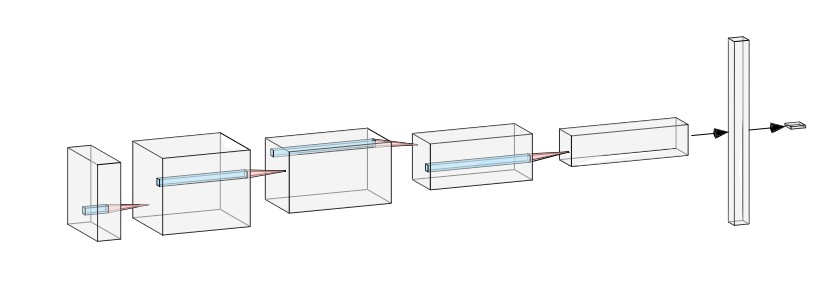
\includegraphics[width=.6\linewidth]{disc.jpg}
    \caption{\small The Structure of Discriminator or Encoder.}
    \label{fig:disc}
\end{figure}

The general description is: input images are fed into $4$ convolutional layers with stride $2$ and padding $same$, then are flatten into a big array before finally sized to the output shape by using $W \cdot X + b$.

\subsection{Generator or Decoder}

The structures of the Generators in GAN and WGAN or the structure of the Decoder in VAE are shown as Figure ~\ref{fig:gen}
\begin{figure}[h]
    \centering
    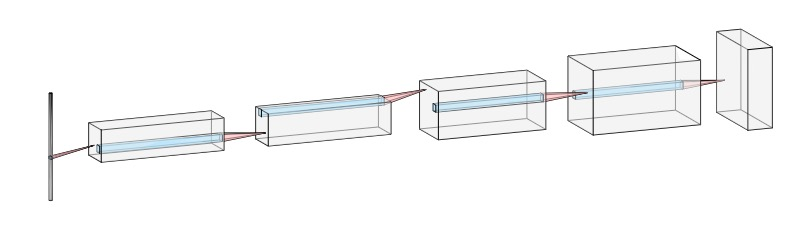
\includegraphics[width=.6\linewidth]{generator.jpg}
    \caption{\small The Structure of Generator or Decoder.}
    \label{fig:gen}
\end{figure}

The general description are: The input latent space is fed into $4$ de-convolutional layers with stride $2$ and padding $same$, with the final layer sizing it back to the same shape as the input image.

\section{MNIST Dataset}

In the following parts, we will first introduce the results and conclusions on the MNIST datasets, then we will go to the CIFAR-10 datasets in the second part.

In the following, $3$ subsections are used for describing the performance of each model as the requirements in the assignment.

In each subsection, the influence of two hyper-parameters (latent size and the number of hidden layers) will be discussed separately.

\subsection{VAE}

\subsubsection{Latent Size}

\subsubsection{Number of Hidden Layers}

\subsection{GAN}

\subsubsection{Latent Size}

First of all, let us take a look at generated images quality of different training time steps. The results are shown as Figure ~\ref{fig:MNIST_GAN_latent}

In MNIST hands-writing datasets, we used 500 epochs to train. There are five rows in each images result. For the $i$-th row, we randomly choose one epoch results in epoch range from $(i-1)*100$ to $i*100$, and we picked 20 images for each row. So the quality of images improves row by row because the model learned better and better with epoch going by. So we only observe the quality of generated images in the last row to analyze the influence of latent size.

To compare the influence of latent size, we fixed the number of hidden layers is $3$, and then compare latent size 10,20,50,100 and 200.

\begin{figure}[h]
    \begin{subfigure}{0.49\textwidth}
    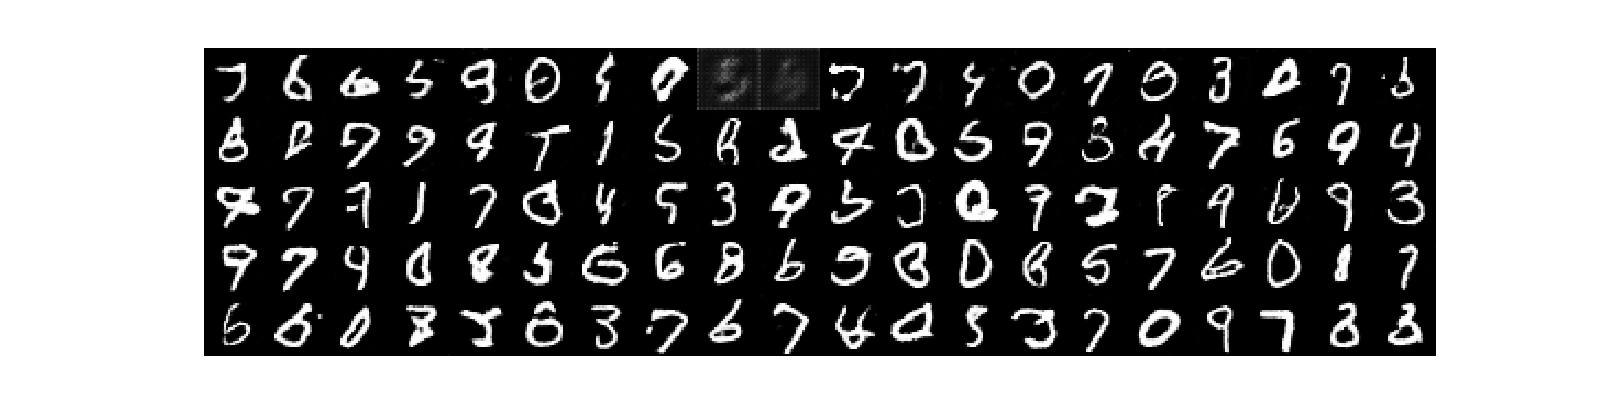
\includegraphics[width=\linewidth]{GAN_MNIST_0_10_256.png}
    \caption{\small Results on latent size 10.} \label{fig:a}
    \end{subfigure}\hspace*{\fill}
    \begin{subfigure}{0.49\textwidth}
    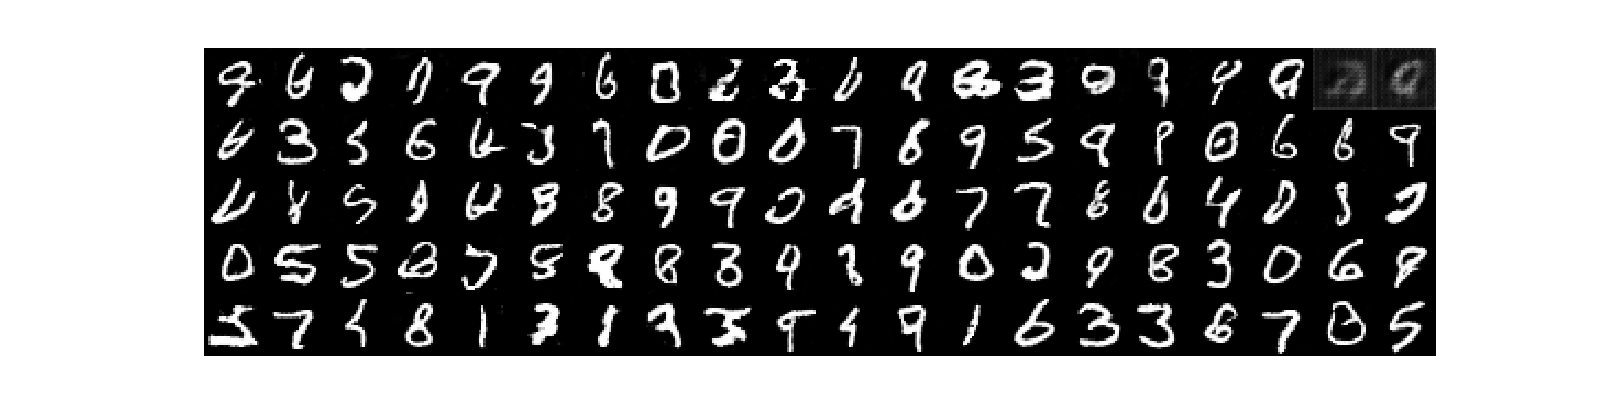
\includegraphics[width=\linewidth]{GAN_MNIST_0_20_256.png}
    \caption{\small Results on latent size 20.} \label{fig:b}
    \end{subfigure}
    
    \medskip
    \begin{subfigure}{0.49\textwidth}
    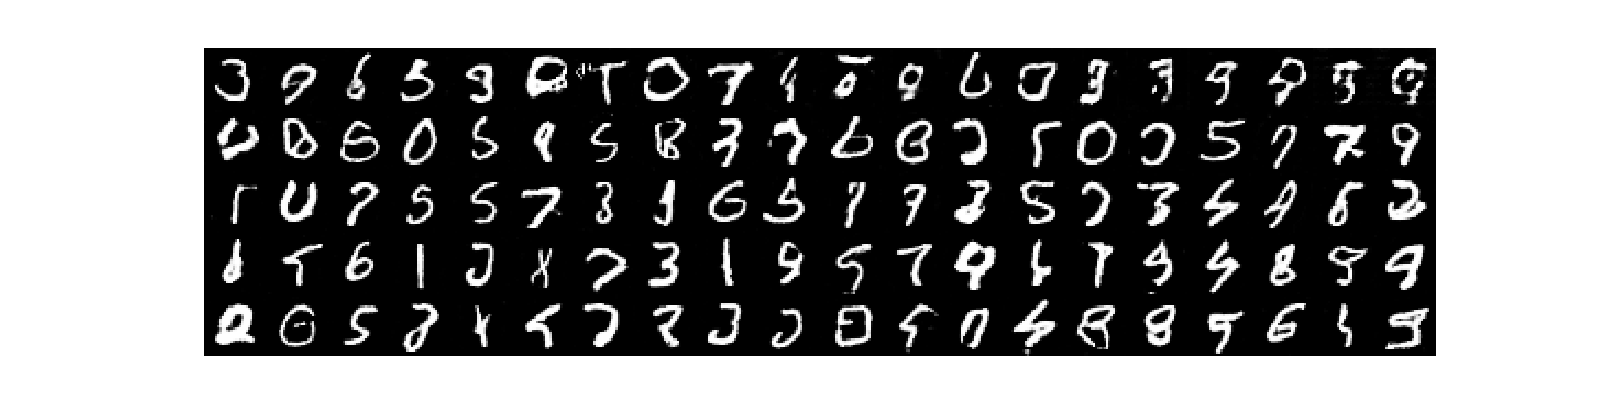
\includegraphics[width=\linewidth]{GAN_MNIST_0_50_256.png}
    \caption{\small Results on latent size 50.} \label{fig:c}
    \end{subfigure}\hspace*{\fill}
    \begin{subfigure}{0.49\textwidth}
    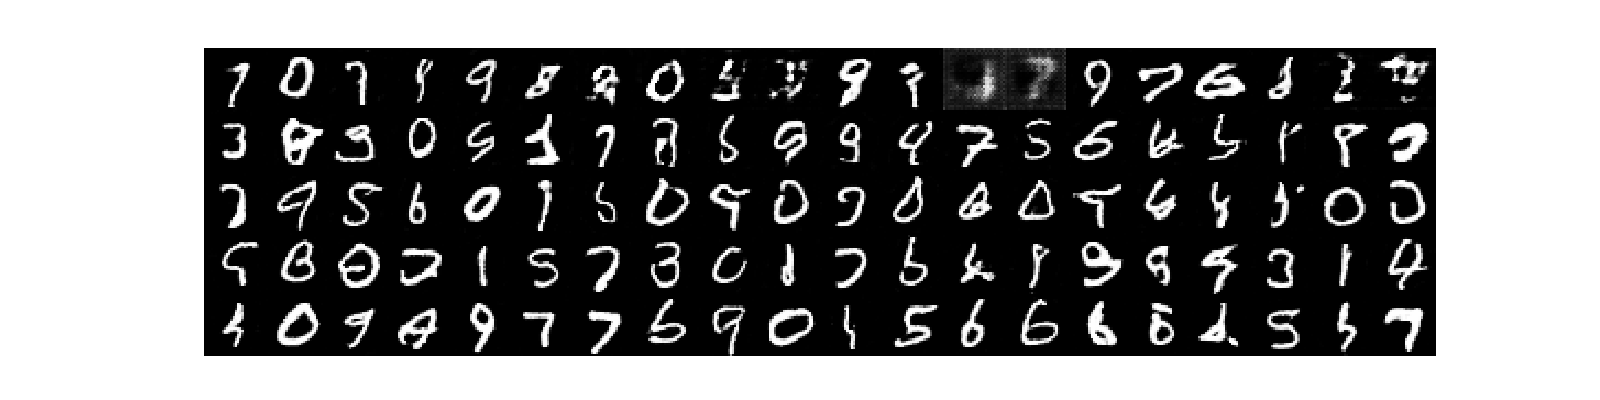
\includegraphics[width=\linewidth]{GAN_MNIST_0_100_256.png}
    \caption{\small Results on latent size 100.} \label{fig:d}
    \end{subfigure}
    
    \medskip
    \begin{subfigure}{0.49\textwidth}
    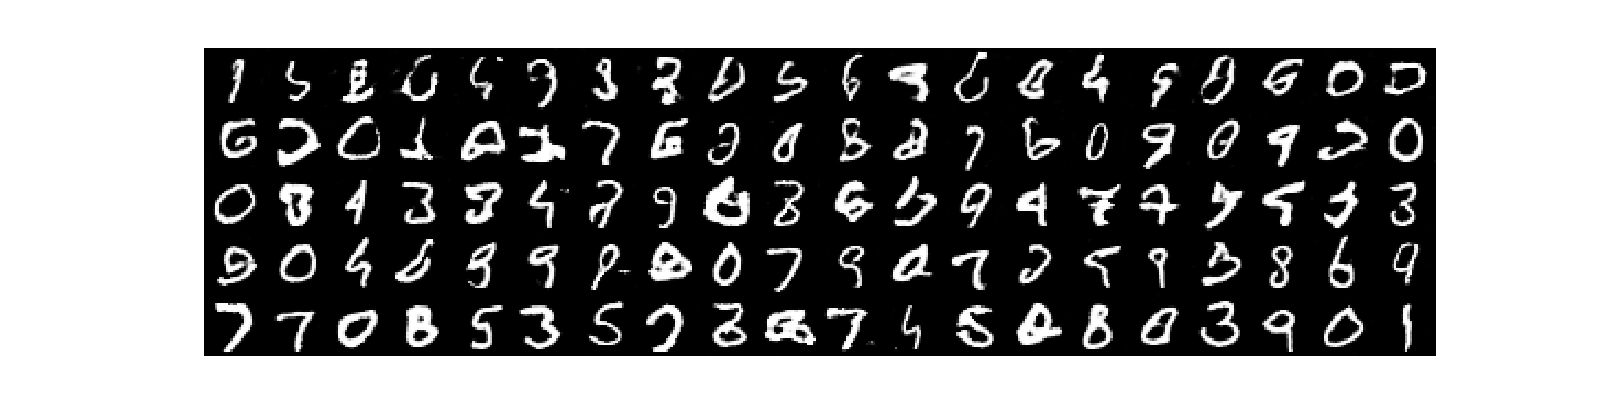
\includegraphics[width=\linewidth]{GAN_MNIST_0_200_256.png}
    \caption{\small Results on latent size 200.} \label{fig:c}
    \end{subfigure}\hspace*{\fill}
    \caption{Influence of the latent size on $5$ models.} \label{fig:MNIST_GAN_latent}
\end{figure}

Intuitively, latent size 100 gets the better result than others. So, too small or too large latent size will reduce the performance of GAN, there is the best result we can get when tuning latent size, and latent size is one of the key hyper-parameters which have to be tuned in real applications.

In order to compare the training effort of the GAN model on different latent space sizes, a plot of generator loss function value is created and plotted as Figure ~\ref{fig:gen_latent}
\begin{figure}[h]
    \centering
    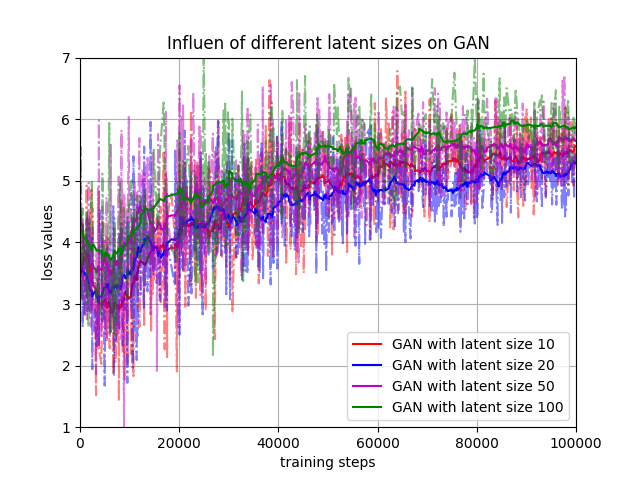
\includegraphics[width=.6\linewidth]{GAN_MNIST_latents.png}
    \caption{\small Different latent size.}
    \label{fig:gen_latent}
\end{figure}



A brief conclusion is drawn as follow,
\begin{itemize}
    \item 
\end{itemize}
 


\subsubsection{Number of Hidden Layers}

First of all, let us take a look at generated images quality of different training time steps. The results are shown as Figure ~\ref{fig:MNIST_GAN_hidden}

To compare the influence of the number of hidden layers, we fixed the latent size is $100$, and then compare the number of hidden layers 3,4 and 5. In this homework, we used 3 hidden layers as the benchmark, and increasing number of hidden layers in both Discriminator and Generator simultaneously. 

\begin{figure}[h]
    \begin{subfigure}{0.49\textwidth}
    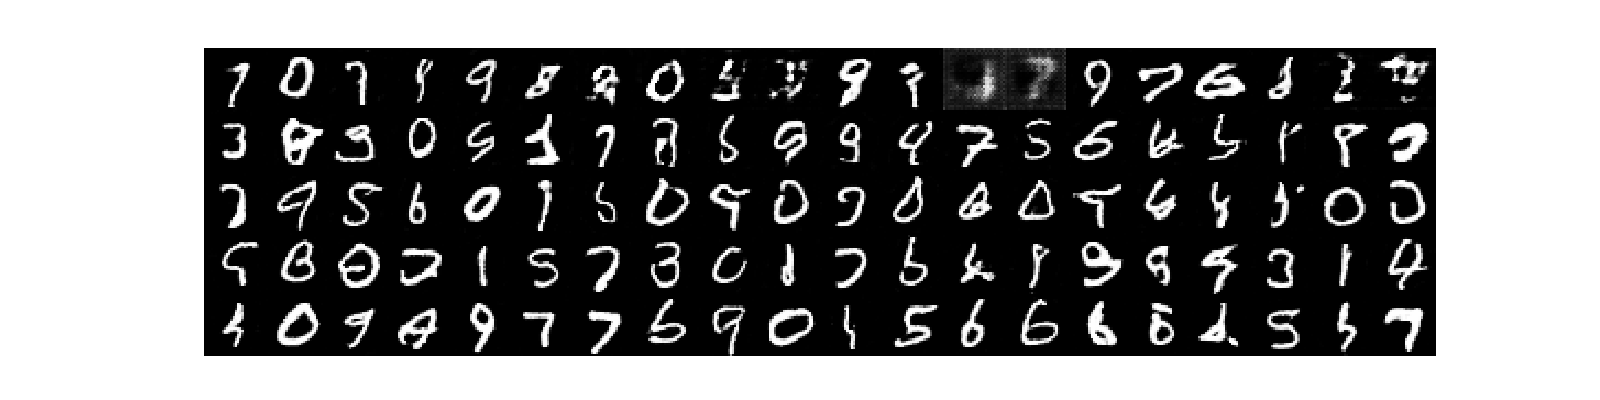
\includegraphics[width=\linewidth]{GAN_MNIST_0_100_256.png}
    \caption{\small Results on 3 hidden layers} \label{fig:a}
    \end{subfigure}\hspace*{\fill}
    \begin{subfigure}{0.49\textwidth}
    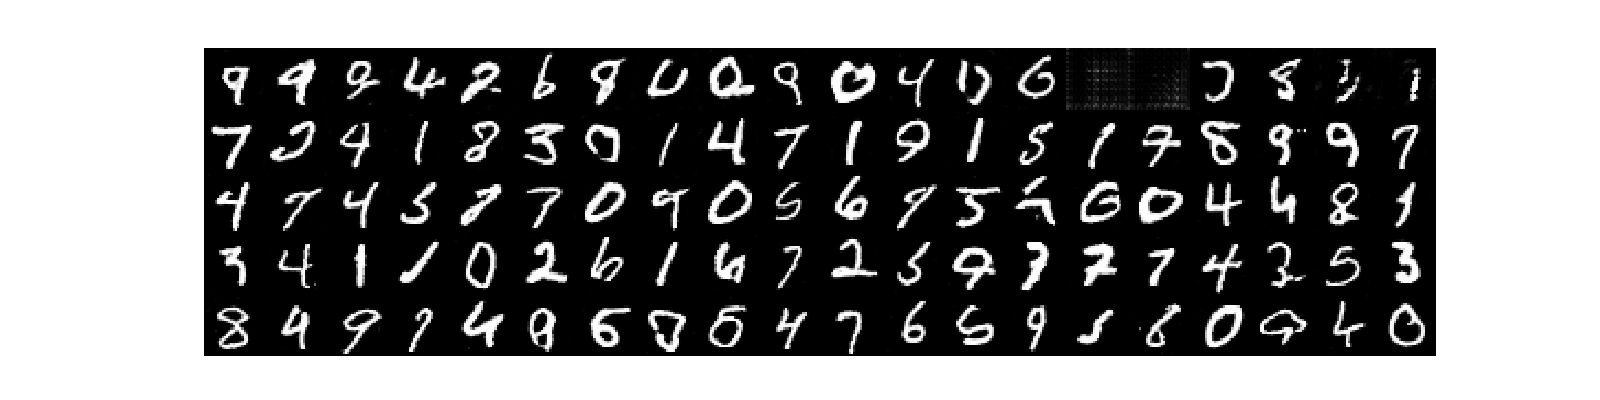
\includegraphics[width=\linewidth]{GAN_MNIST_1_100_256.png}
    \caption{\small Results on 4 hidden layers} \label{fig:b}
    \end{subfigure}

    \medskip
    \begin{subfigure}{0.49\textwidth}
    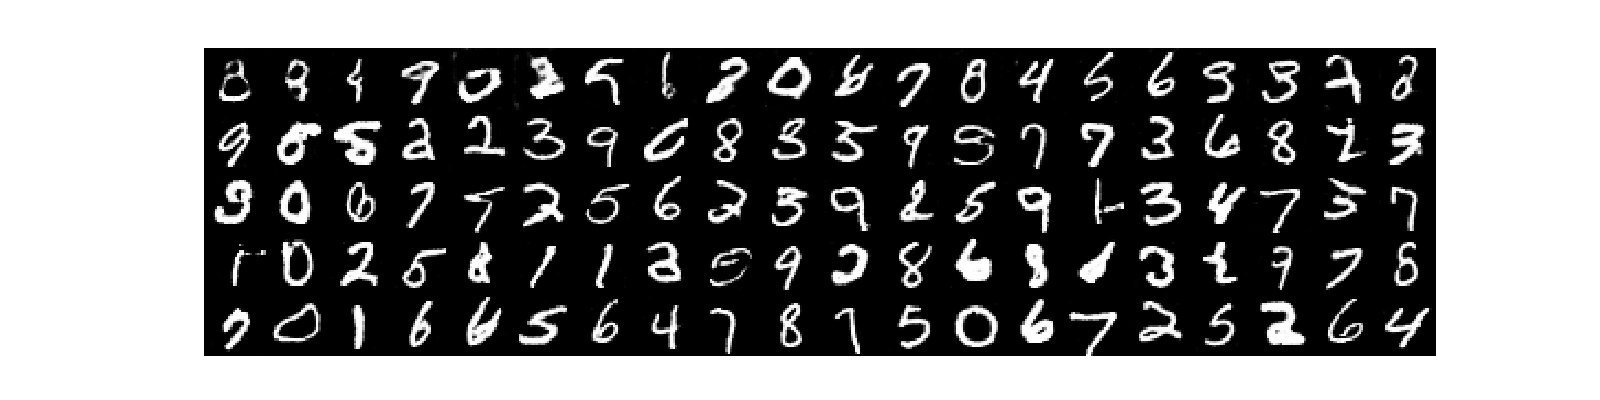
\includegraphics[width=\linewidth]{GAN_MNIST_2_100_256.png}
    \caption{\small Results on 5 hidden layers} \label{fig:c}
    \end{subfigure}\hspace*{\fill}
    \caption{Influence of the number of hidden layers on $3$ models.} \label{fig:MNIST_GAN_hidden}
\end{figure}

Intuitively, 5 hidden layers gets the better result than others. So, adding hidden layers can improve the performance of the model in this case, but too much hidden layers will occur over-fitting. So, the number of hidden layers is also one of the key hyper-parameters which have to be tuned in real applications.

In order to compare the training effort of the GAN model on different number of hidden layers, a plot of generator loss function value is created and plotted as Figure ~\ref{fig:gen_hidden}
\begin{figure}[h]
    \centering
    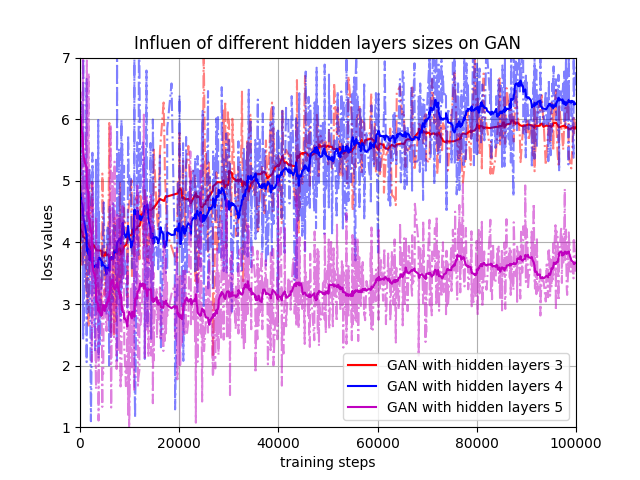
\includegraphics[width=.6\linewidth]{GAN_MNIST_hidden.png}
    \caption{\small Different number of hidden layers.}
    \label{fig:gen_hidden}
\end{figure}



A brief conclusion is drawn as follow,
\begin{itemize}
    \item 
\end{itemize}

\textbf{Hyper-parameters settings}: The hyper-parameters we used to get these results are shown as follow,
\begin{table}[h]
        \centering
        \vspace{\baselineskip}
        \caption{All relative parameters values.}\label{T:parameters}
      \begin{tabular}{cc}
        \hline
        Parameter & Value\\
        \hline
        learning rate & 0.0001\\
        optimizer & Adam\\
        \hline
      \end{tabular}
\end{table}
%%%%%%%%%%%%%%%%%%%%%%%%%%%%%%%%%%%%%%%%%%%%%%%%%%%%
\subsection{WGAN}

The difference of GAN and WGAN is cost function, and they use different cost function to find the optimal solution. So converting GAN to WGAN needs $3$ operations:
\begin{itemize}
    \item Remove sigmoid activation function of the last dense layer in discriminator
    \item Change loss function of both generator and discriminator
    \item Use weight clip when updating the weight or gradient penalty, which is WGAN-GP.
\end{itemize}

\subsubsection{Latent Size}

First of all, let us take a look at generated images quality of different training time steps. The results are shown as Figure ~\ref{fig:MNIST_WGAN_latent}

\begin{figure}[h]
    \begin{subfigure}{0.49\textwidth}
    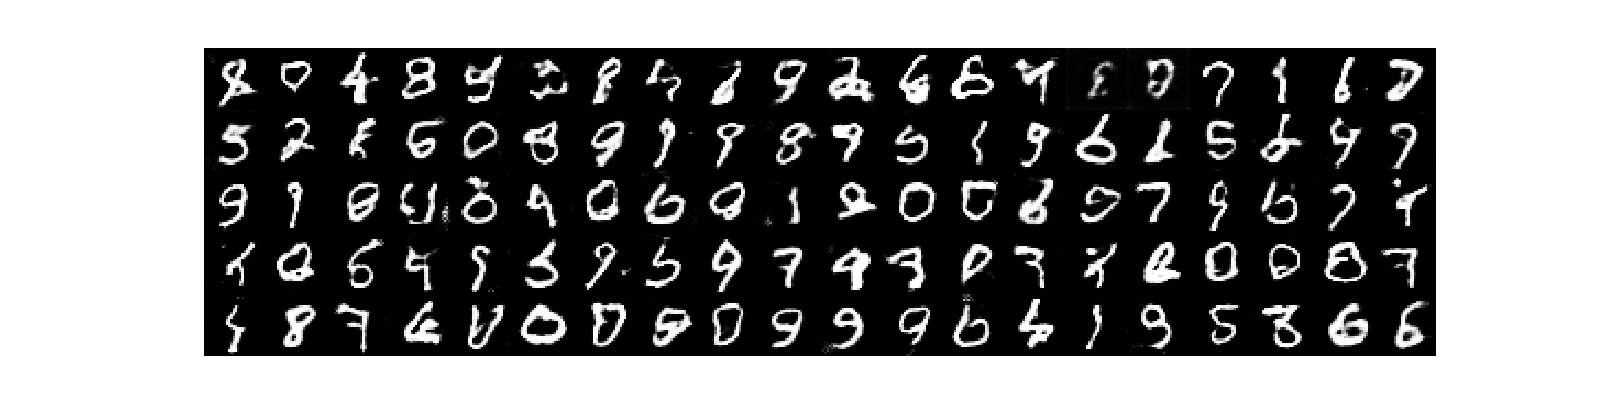
\includegraphics[width=\linewidth]{WGAN_MNIST_0_10_256.png}
    \caption{\small Results on latent size 10.} \label{fig:a}
    \end{subfigure}\hspace*{\fill}
    \begin{subfigure}{0.49\textwidth}
    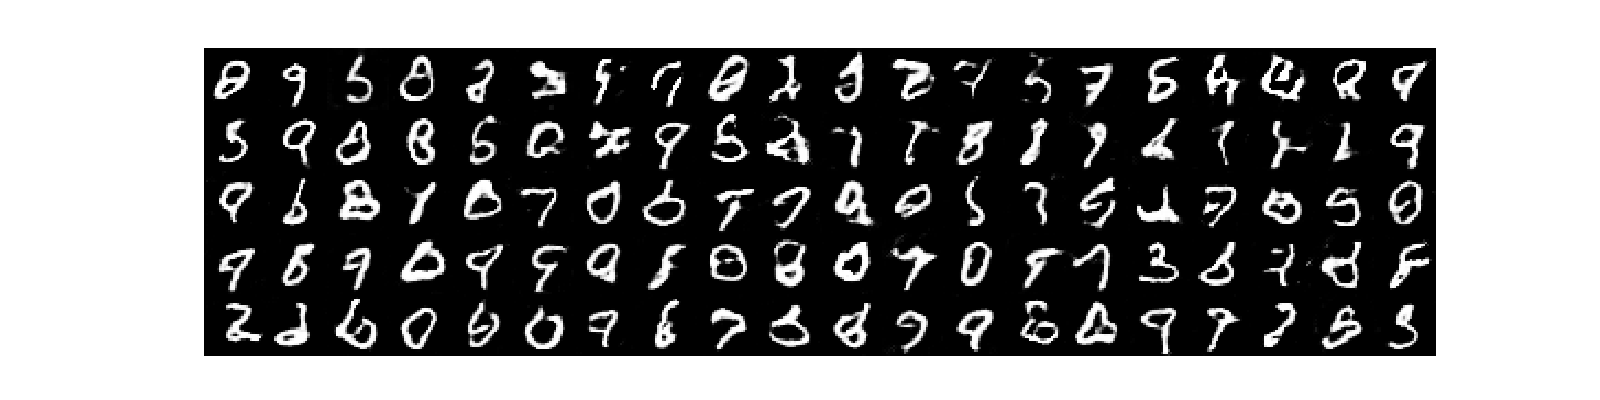
\includegraphics[width=\linewidth]{WGAN_MNIST_0_20_256.png}
    \caption{\small Results on latent size 20.} \label{fig:b}
    \end{subfigure}
    
    \medskip
    \begin{subfigure}{0.49\textwidth}
    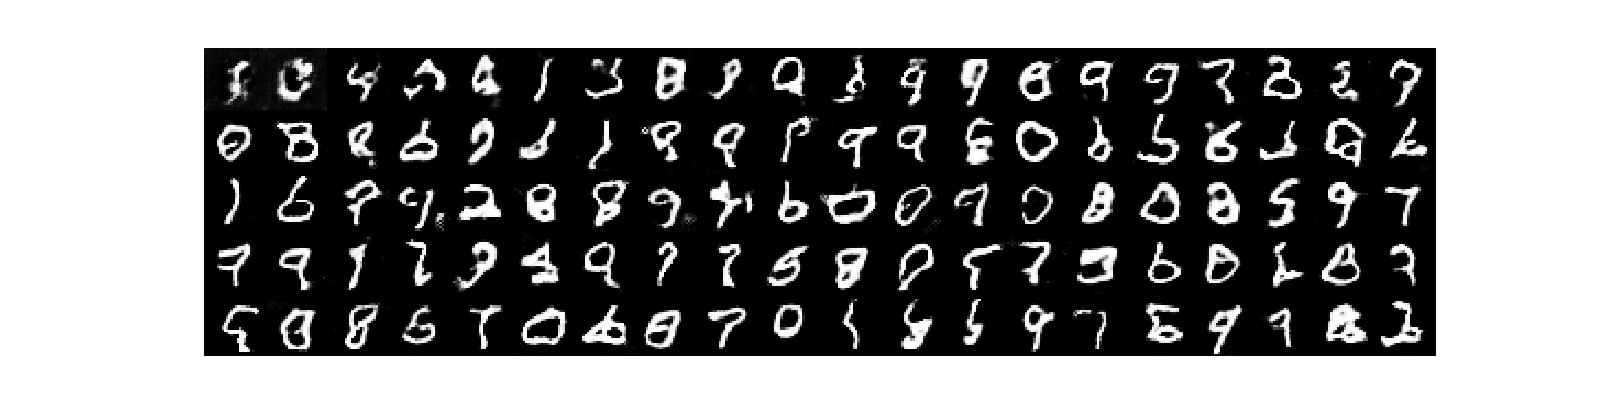
\includegraphics[width=\linewidth]{WGAN_MNIST_0_50_256.png}
    \caption{\small Results on latent size 50.} \label{fig:c}
    \end{subfigure}\hspace*{\fill}
    \begin{subfigure}{0.49\textwidth}
    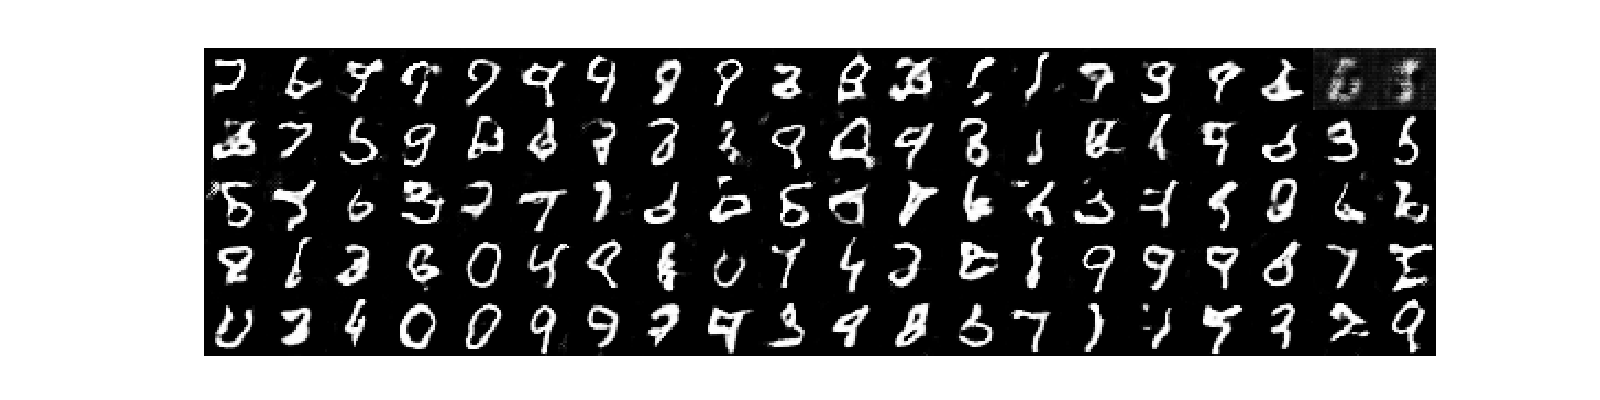
\includegraphics[width=\linewidth]{WGAN_MNIST_0_100_256.png}
    \caption{\small Results on latent size 100.} \label{fig:d}
    \end{subfigure}
    
    \medskip
    \begin{subfigure}{0.49\textwidth}
    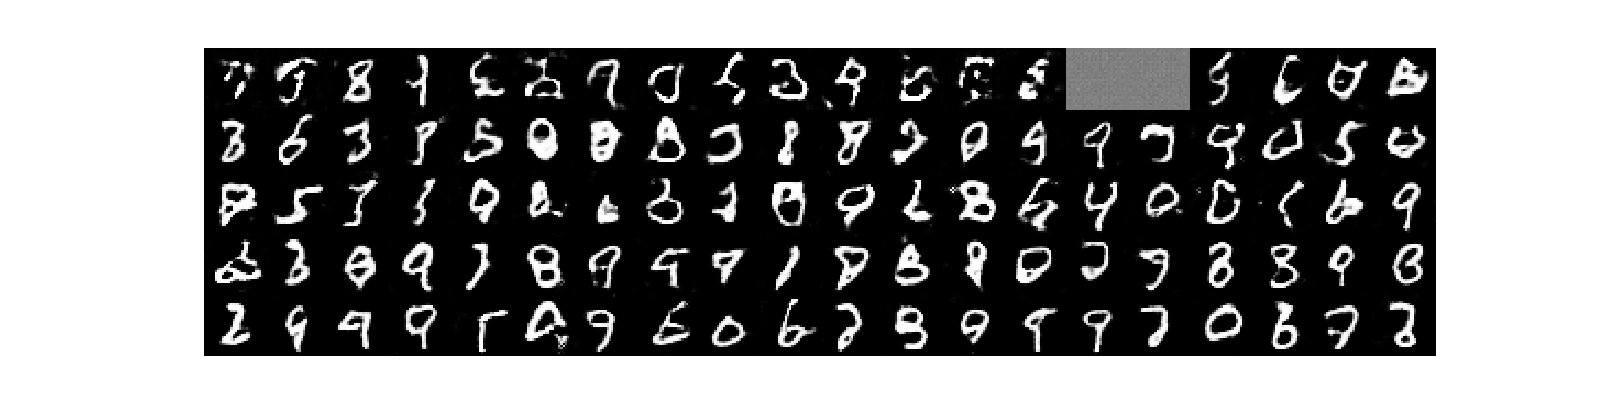
\includegraphics[width=\linewidth]{WGAN_MNIST_0_200_256.png}
    \caption{\small Results on latent size 200.} \label{fig:c}
    \end{subfigure}\hspace*{\fill}
    \caption{Influence of the latent size on $5$ models.} \label{fig:MNIST_GAN_latent}
\end{figure}

Intuitively, latent size 200 gets the better result than others, which is different to the best latent size of GAN, so for each kind of GAN model, there is one matching best latent size to reach the best performance.

In order to compare the training effort of the WGAN model on different latent space sizes, a plot of generator loss function value is created and plotted as Figure ~\ref{fig:wgen_latent}
\begin{figure}[h]
    \centering
    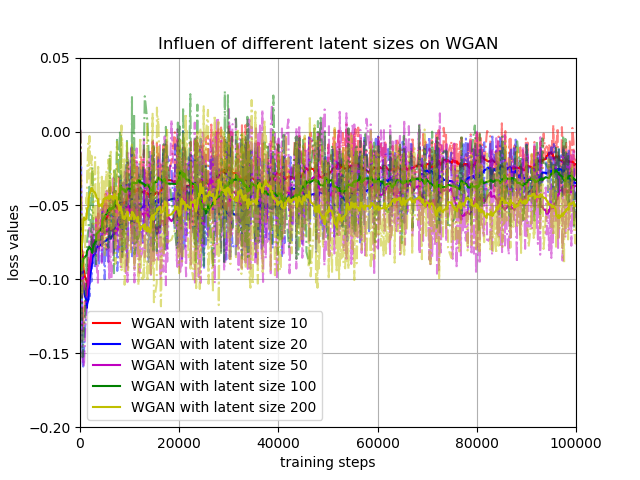
\includegraphics[width=.6\linewidth]{WGAN_MNIST_latents.png}
    \caption{\small Different latent size.}
    \label{fig:wgen_latent}
\end{figure}



A brief conclusion is drawn as follow,
\begin{itemize}
    \item 
\end{itemize}
 


\subsubsection{Number of Hidden Layers}

First of all, let us take a look at generated images quality of different training time steps. The results are shown as Figure ~\ref{fig:MNIST_WGAN_hidden}

Increasing number of hidden layers in both Critic and Generator simultaneously. 

\begin{figure}[h]
    \begin{subfigure}{0.49\textwidth}
    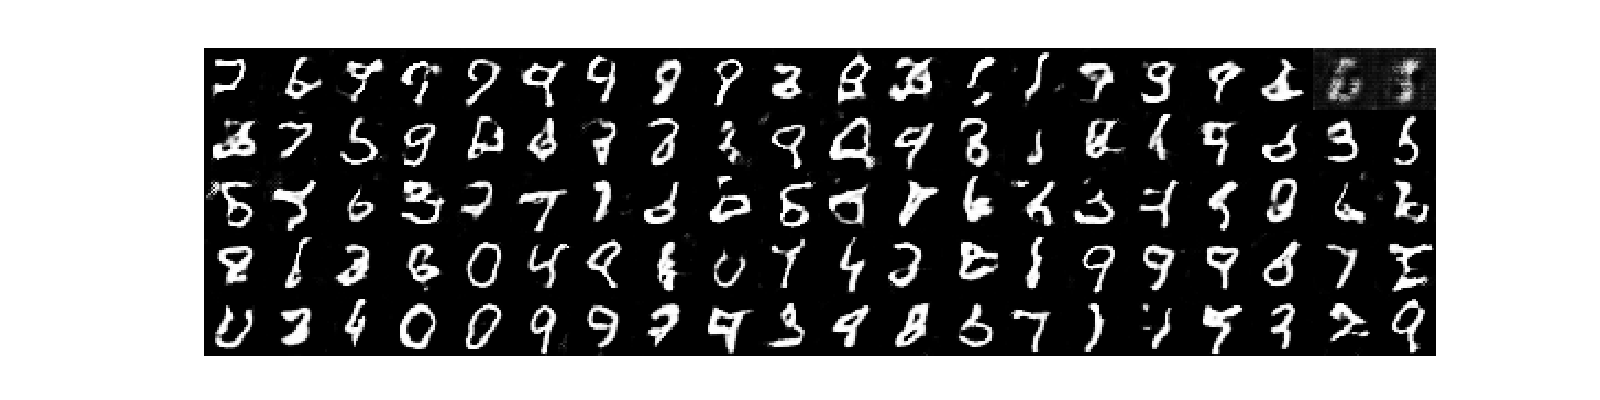
\includegraphics[width=\linewidth]{WGAN_MNIST_0_100_256.png}
    \caption{\small Results on 3 hidden layers} \label{fig:a}
    \end{subfigure}\hspace*{\fill}
    \begin{subfigure}{0.49\textwidth}
    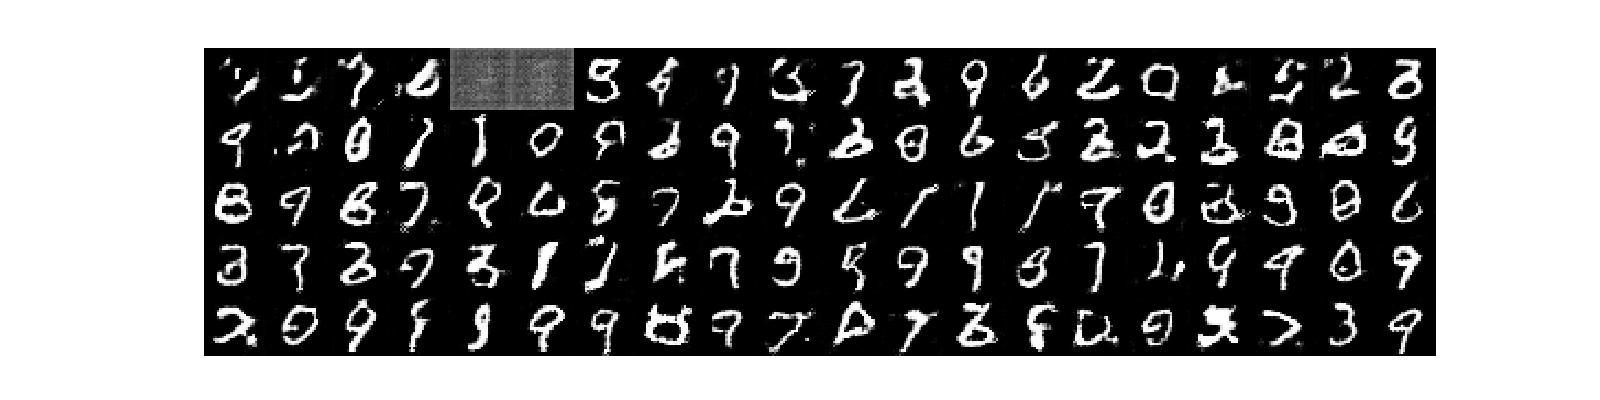
\includegraphics[width=\linewidth]{WGAN_MNIST_1_100_256.png}
    \caption{\small Results on 4 hidden layers} \label{fig:b}
    \end{subfigure}

    \medskip
    \begin{subfigure}{0.49\textwidth}
    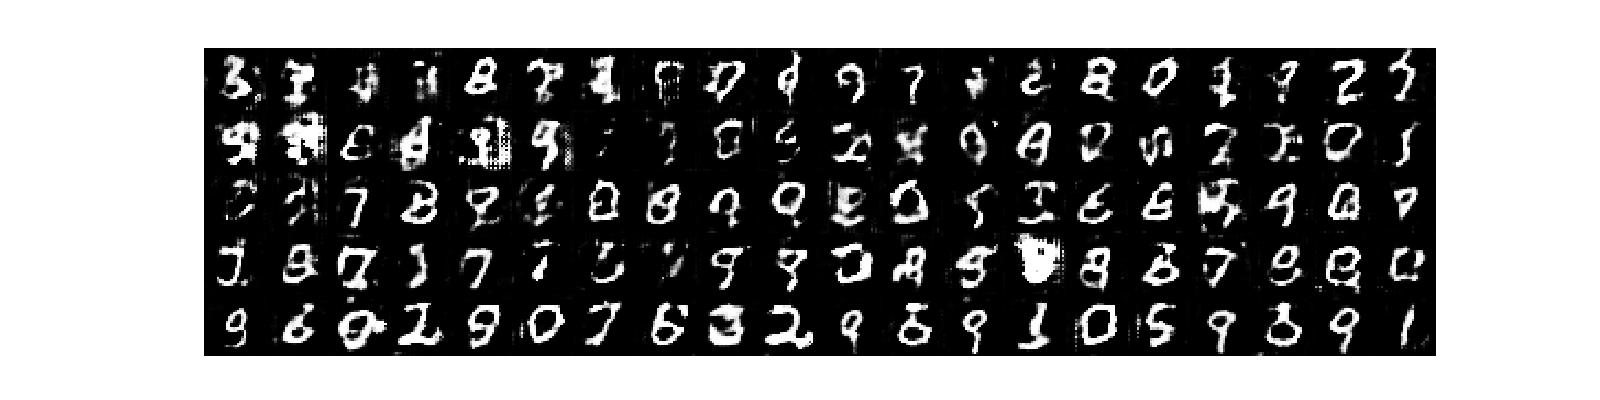
\includegraphics[width=\linewidth]{WGAN_MNIST_2_100_256.png}
    \caption{\small Results on 5 hidden layers} \label{fig:c}
    \end{subfigure}\hspace*{\fill}
    \caption{Influence of the number of hidden layers on $3$ models.} \label{fig:MNIST_WGAN_hidden}
\end{figure}

Intuitively, 3 hidden layers gets the better result than others, which is different to the best number of hidden layers of GAN. So, for each kind of GAN model, there is one matching best number of hidden layers to reach the best performance.

In order to compare the training effort of the WGAN model on different number of hidden layers, a plot of generator loss function value is created and plotted as Figure ~\ref{fig:wgen_hidden}
\begin{figure}[h]
    \centering
    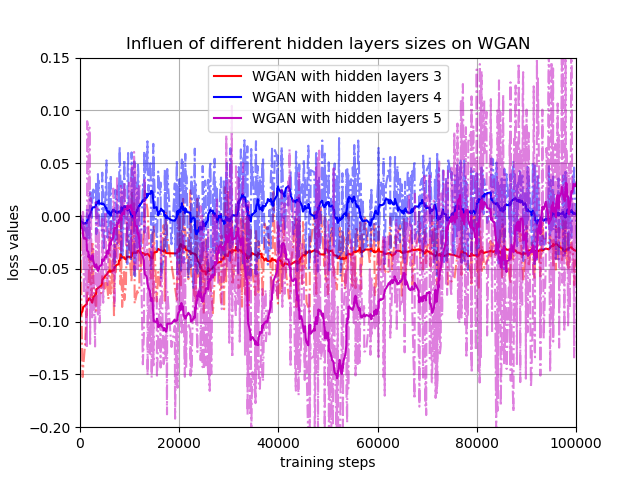
\includegraphics[width=.6\linewidth]{WGAN_MNIST_hidden.png}
    \caption{\small Different number of hidden layers.}
    \label{fig:wgen_hidden}
\end{figure}



A brief conclusion is drawn as follow,
\begin{itemize}
    \item 
\end{itemize}

\textbf{Hyper-parameters settings}: The hyper-parameters we used to get these results are shown as follow,
\begin{table}[h]
        \centering
        \vspace{\baselineskip}
        \caption{All relative parameters values.}\label{T:parameters}
      \begin{tabular}{cc}
        \hline
        Parameter & Value\\
        \hline
        learning rate & 0.00001\\
        optimizer & RMSprop\\
        weight clip & 0.01\\
        \hline
      \end{tabular}
\end{table}


\newpage
\section{CIFAR-10 Dataset}

Before dive into the content, we firstly have to apologize for the low quality of the generated images. We have tried several network structures and tuned hyper-parameters multi-times. Also, since the time is limited, we decided to set the training epochs as $1000$. The results we are currently presenting in this report is possibly the best we can get.

Back to the report, this section is separated into $3$ subsections with each model occupying one subsection.

\subsection{VAE}

\subsubsection{Latent Size}

\subsubsection{Number of Hidden Layers}

\subsection{GAN}

\subsubsection{Latent Size}

\subsubsection{Number of Hidden Layers}

\subsection{WGAN}

\subsubsection{Latent Size}

\subsubsection{Number of Hidden Layers}


Some experience of building up hidden layers structure and tuning hyper-parameters:
\begin{itemize}
    \item 
\end{itemize}



% \begin{verbatim}
% {
%     str(word1) : 0,
%     str(word2) : 1,
%     ...
% }
% \end{verbatim}


% \begin{figure}[h]
%     \centering
%     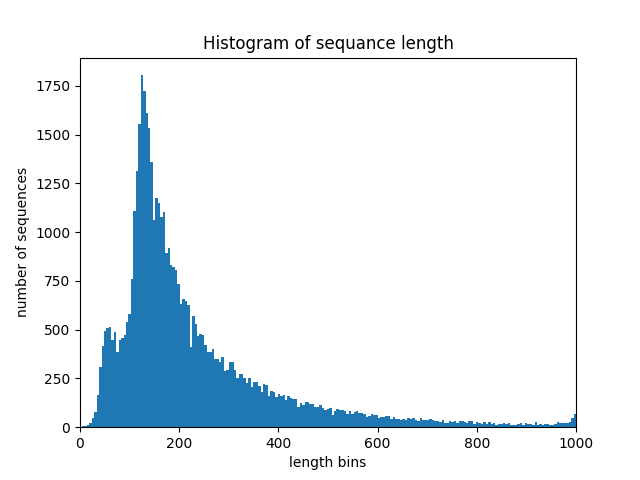
\includegraphics[width=.6\linewidth]{lengthdistribution.png}
%     \caption{\small Distribution of dataset file lengths.}
%     \label{fig:length}
% \end{figure}


% \begin{figure}[h]
%     \begin{subfigure}{0.49\textwidth}
%     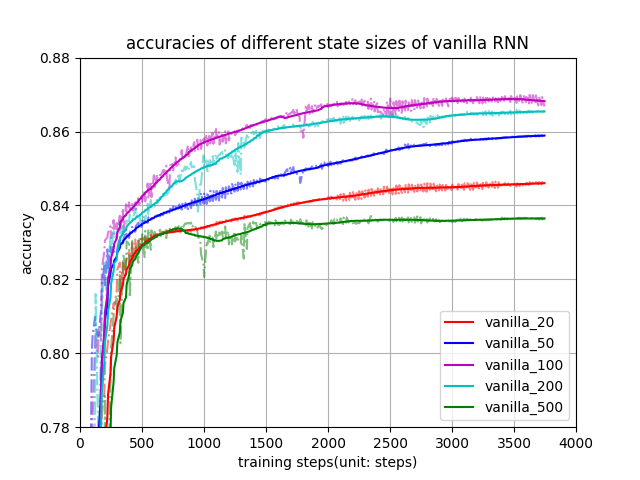
\includegraphics[width=\linewidth]{vanilla_acc.png}
%     \caption{\small Results on accuracy of Vanilla RNN.} \label{fig:a}
%     \end{subfigure}\hspace*{\fill}
%     \begin{subfigure}{0.49\textwidth}
%     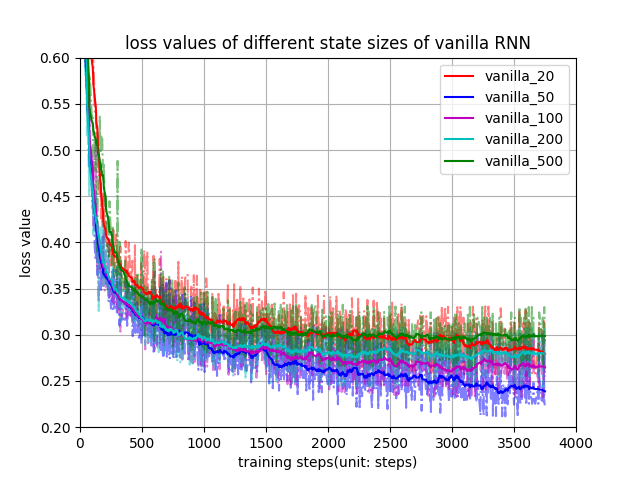
\includegraphics[width=\linewidth]{vanilla_loss.png}
%     \caption{\small Results on loss of Vanilla RNN.} \label{fig:b}
%     \end{subfigure}
    
%     \medskip
%     \begin{subfigure}{0.49\textwidth}
%     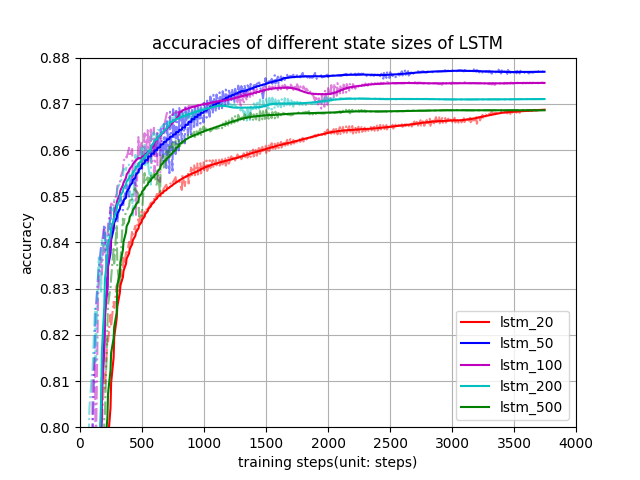
\includegraphics[width=\linewidth]{lstm_acc.png}
%     \caption{\small Results on accuracy of LSTM.} \label{fig:c}
%     \end{subfigure}\hspace*{\fill}
%     \begin{subfigure}{0.49\textwidth}
%     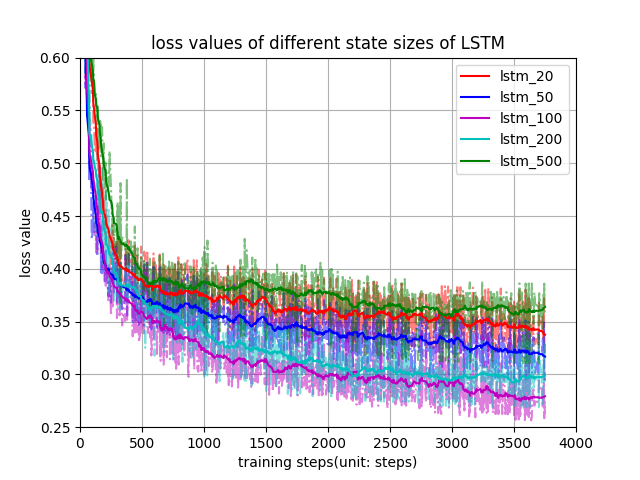
\includegraphics[width=\linewidth]{lstm_loss.png}
%     \caption{\small Results on loss of LSTM.} \label{fig:d}
%     \end{subfigure}
%     \caption{Influence of state dimensions on $2$ models.} \label{fig:BN}
% \end{figure}

% \begin{figure}[h]
%     \centering
%     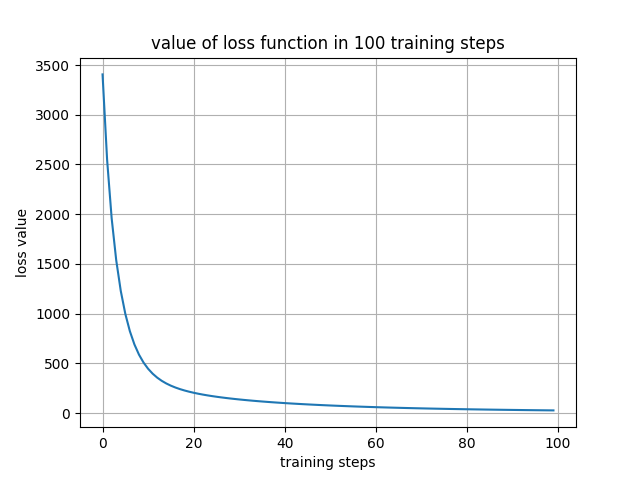
\includegraphics[width=.6\linewidth]{assignment1_question1.png}
%     \caption{\small Results of back propagation.}
%     \label{fig:experiment}
% \end{figure}


% \begin{table}[h]
%         \centering
%         \vspace{\baselineskip}
%         \caption{All relative parameters values.}\label{T:parameters}
%       \begin{tabular}{cc}
%         \hline
%         Parameter & Value\\
%         \hline
%         N (number of inputs) & 100\\
%         K (input dimensions) & 5\\
%         optimization & Gradient Descent\\
%         \hline
%       \end{tabular}
% \end{table}

% \begin{figure}[h]
%     \begin{subfigure}{0.32\textwidth}
%     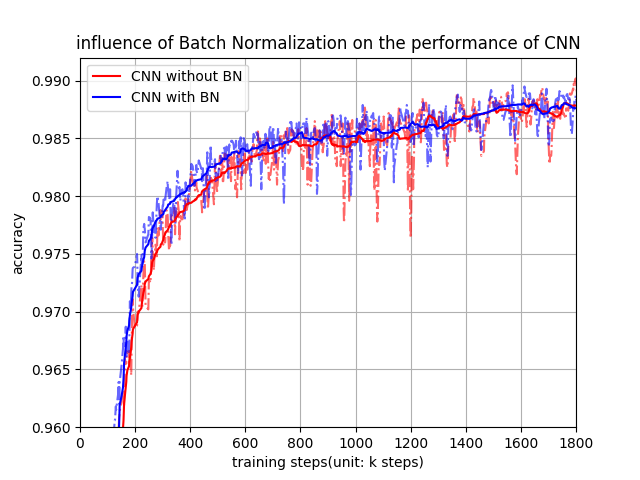
\includegraphics[width=\linewidth]{CNN_BN_acc.png}
%     \caption{\small Influence of BN on accuracy of CNN} \label{fig:a}
%     \end{subfigure}\hspace*{\fill}
%     \begin{subfigure}{0.32\textwidth}
%     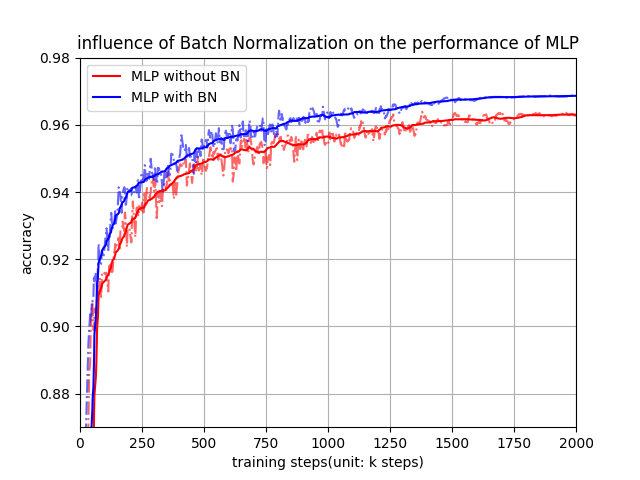
\includegraphics[width=\linewidth]{MLP_BN_acc.png}
%     \caption{\small Influence of BN on accuracy of MLP} \label{fig:b}
%     \end{subfigure}
%     \begin{subfigure}{0.32\textwidth}
%     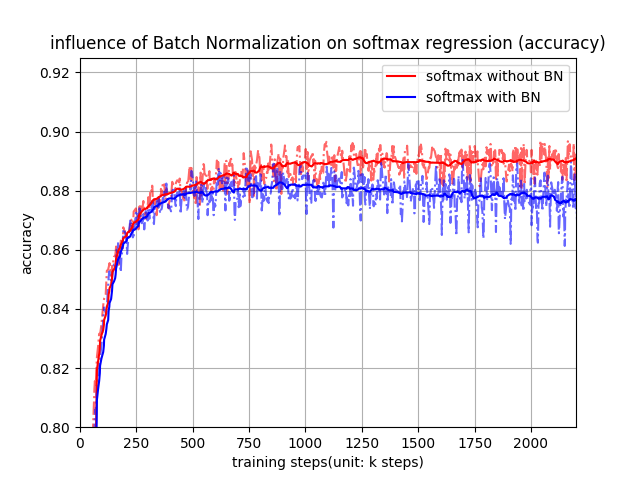
\includegraphics[width=\linewidth]{softmax_BN_acc.png}
%     \caption{\small Influence of BN on accuracy of soft-max} \label{fig:b}
%     \end{subfigure}
    
%     \medskip
%     \begin{subfigure}{0.32\textwidth}
%     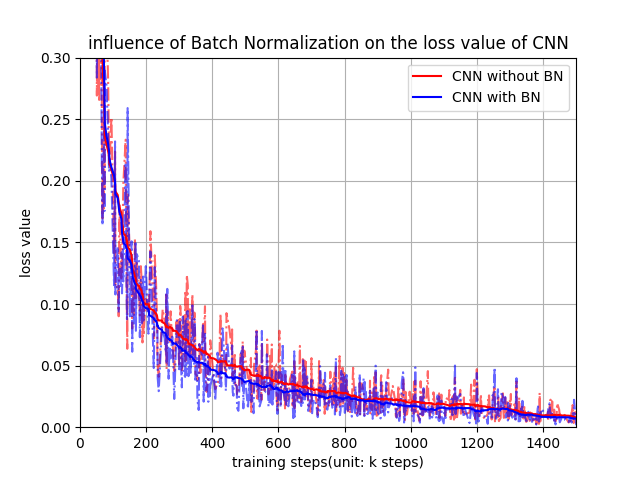
\includegraphics[width=\linewidth]{CNN_BN_loss.png}
%     \caption{\small Influence of BN on loss of CNN} \label{fig:c}
%     \end{subfigure}\hspace*{\fill}
%     \begin{subfigure}{0.32\textwidth}
%     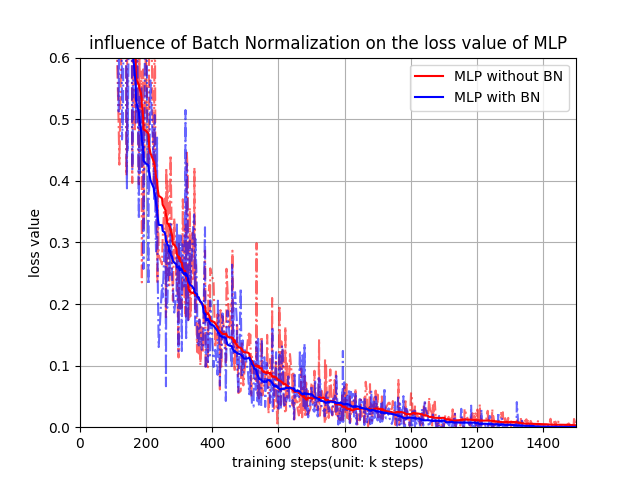
\includegraphics[width=\linewidth]{MLP_BN_loss.png}
%     \caption{\small Influence of BN on loss of MLP} \label{fig:d}
%     \end{subfigure}
%     \begin{subfigure}{0.32\textwidth}
%     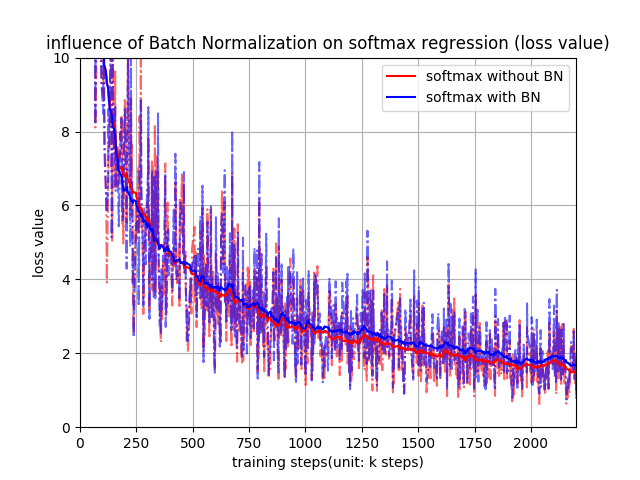
\includegraphics[width=\linewidth]{softmax_BN_loss.png}
%     \caption{\small Influence of BN on loss of soft-max} \label{fig:d}
%     \end{subfigure}
%     \caption{Influence of Batch Normalization on $3$ models.} \label{fig:BN}
% \end{figure}


% \begin{figure}[h]
% \centering
% \begin{subfigure}{.45\textwidth}
%   \centering
%   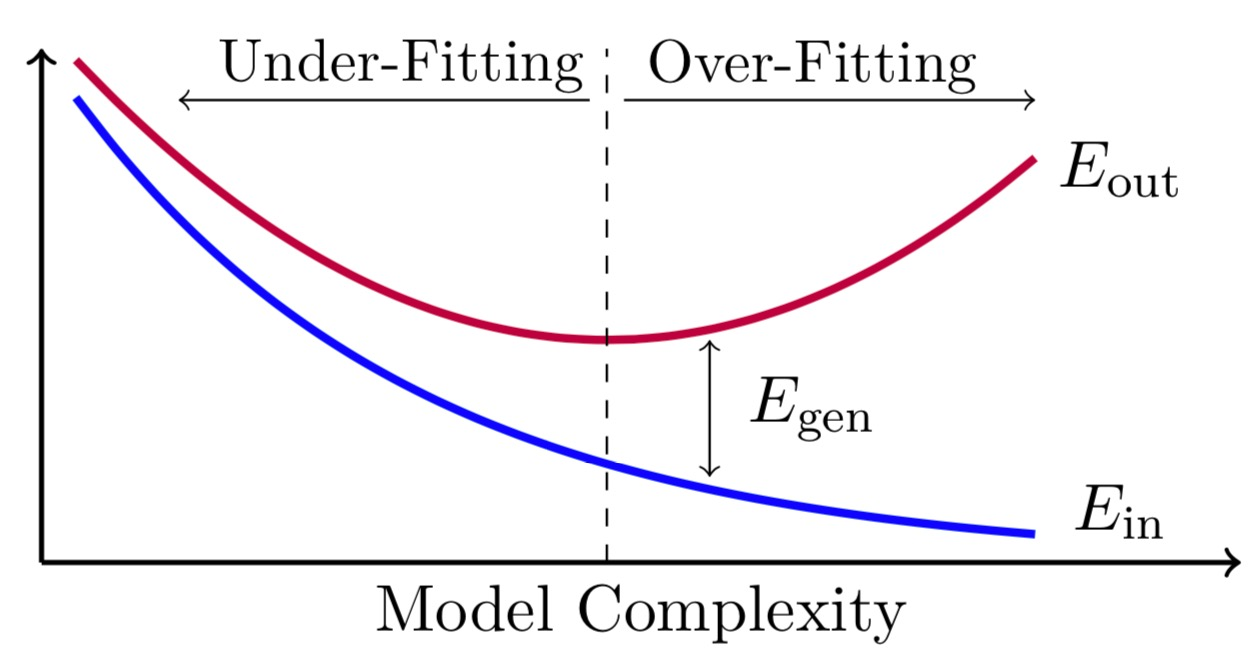
\includegraphics[width=.9\linewidth]{d_txtbook.jpg}
%   \caption{\small figure from textbook}
%   \label{fig:sub1}
% \end{subfigure}%
% \begin{subfigure}{.45\textwidth}
%   \centering
%   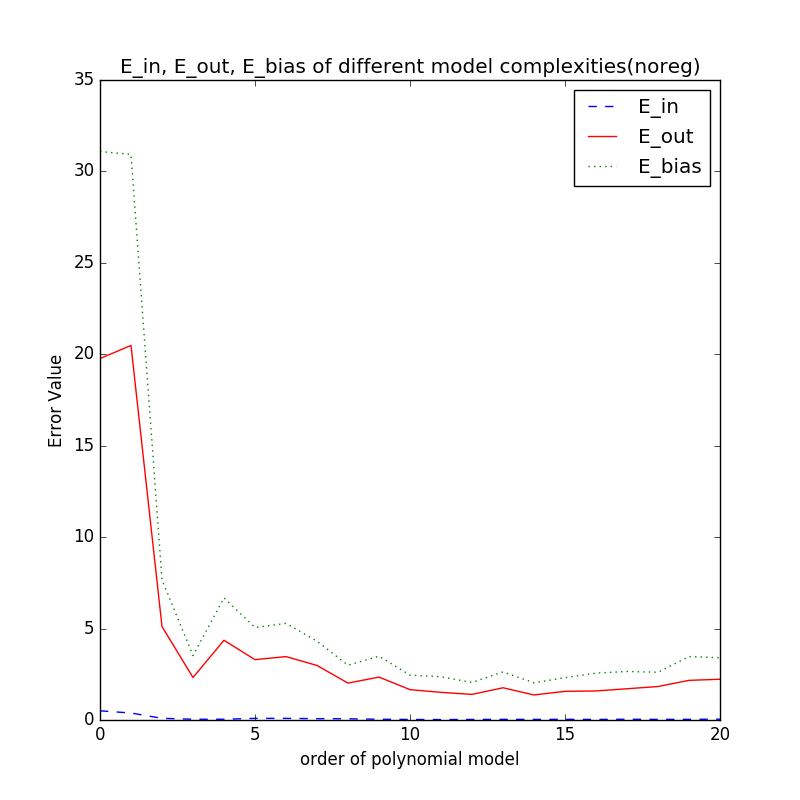
\includegraphics[width=.9\linewidth]{test_d_noreg.png}
%   \caption{\small figure of test}
%   \label{fig:sub2}
% \end{subfigure}
% \caption{\small Results of complexities.}
% \label{fig:complex_nonreg}
% \end{figure}


\end{document}